\begin{figure*}[t]
    \centering
    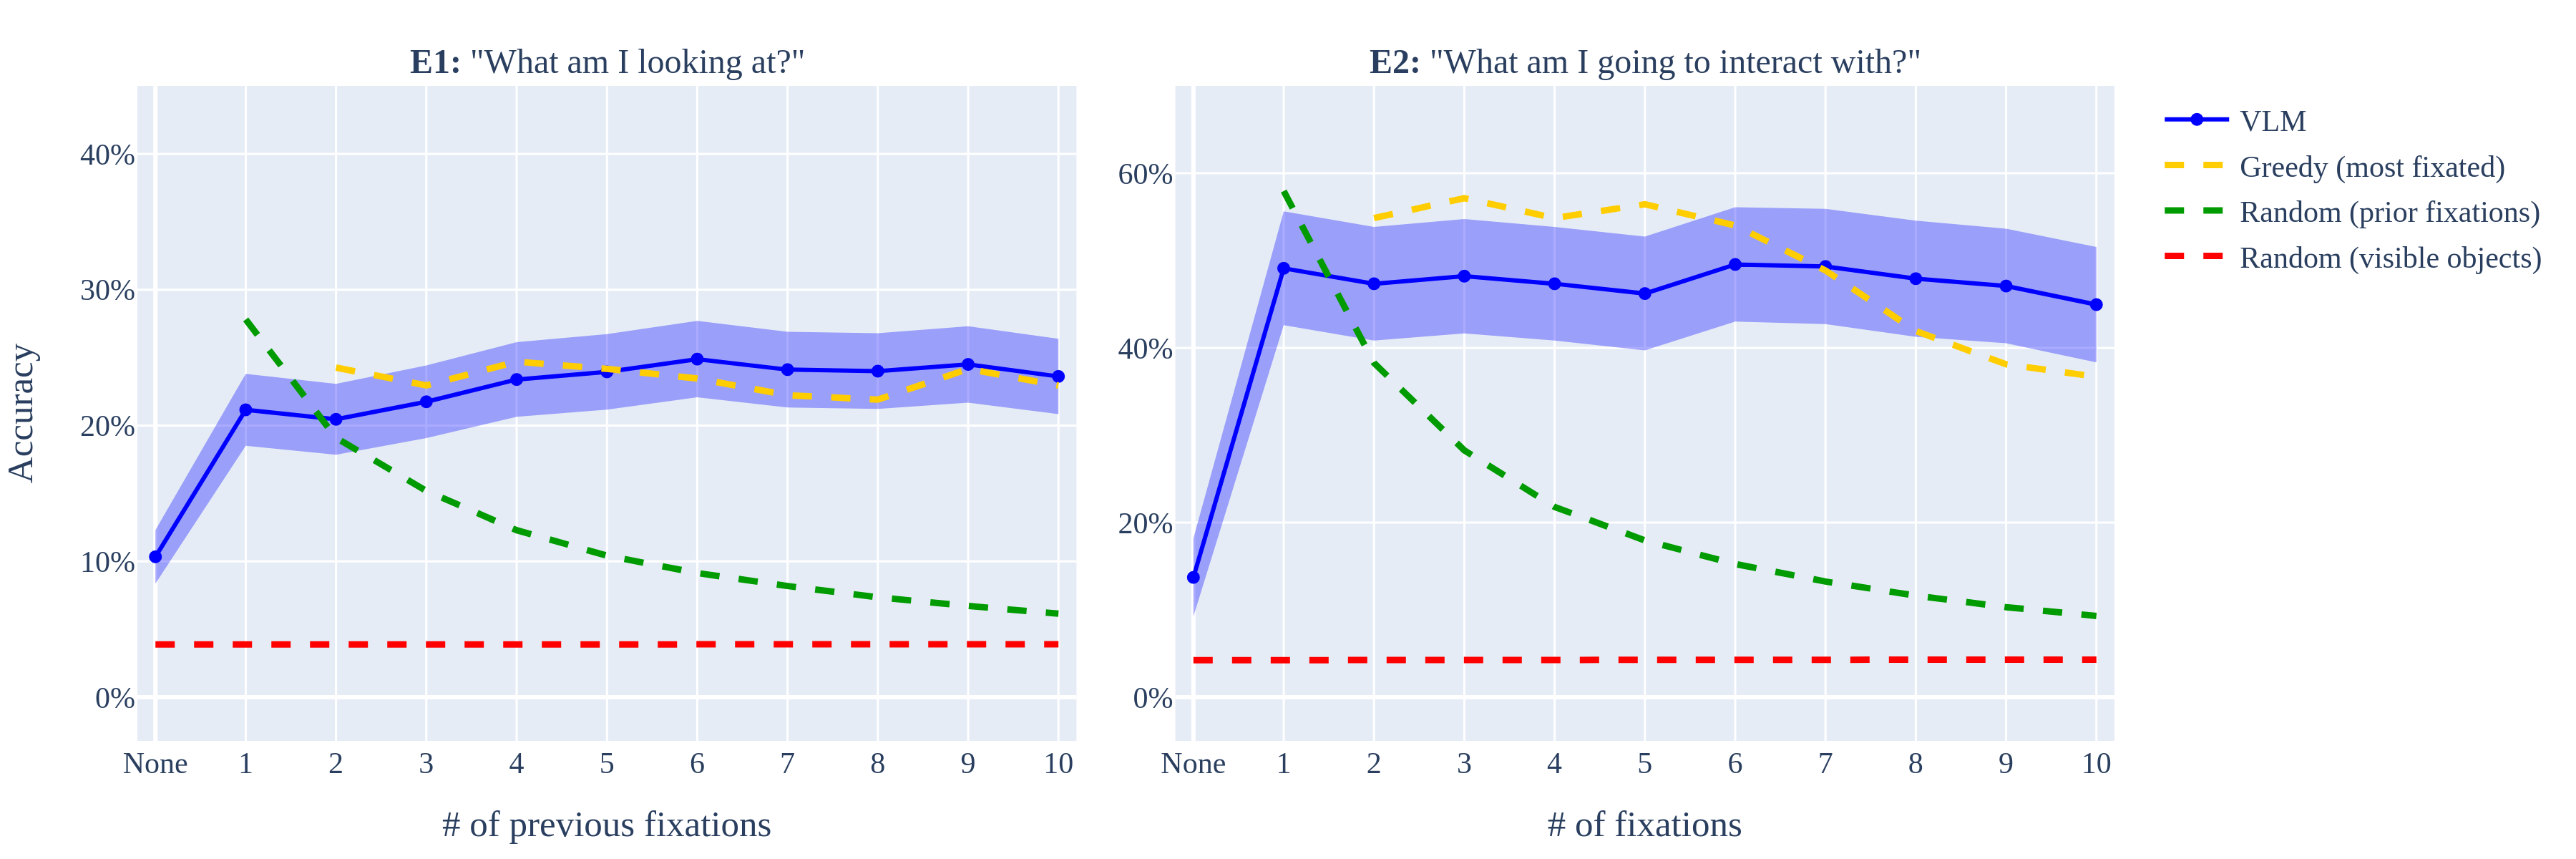
\includegraphics[width=\linewidth]{figures/e1e2.png}
    \caption{Experiments where prior gaze fixation contents are supplied to a VLM along with egocentric images.  When many fixations are given as context, the model can synthesize image + gaze information to outperform a greedy baseline that only considers contents from the prompt. The error surfaces in light blue represent 95\% confidence intervals.}
    \label{fig:e1e2}
\end{figure*}

\section{Eye Tracking Context in Vision-language Model Queries}

To begin to explore the value that ET signals can provide in contextual AI systems, we model experiments which reflect potential end-to-end contextual AI systems.  In these experiments, we build up historical context by creating timelines of past fixations on physical objects.  This context is included in VLM queries to measure positive impacts on model understanding.  Our baseline comparison is a VLM query which uses only the egocentric image as added context (similar to a Ray-Ban Meta or Google Ask Photos query).

\subsection{Methodology}

The Meta Llama 3.2 90B VLM\footnote{\url{https://ai.meta.com/blog/llama-3-2-connect-2024-vision-edge-mobile-devices/}}~\cite{grattafiori_llama_2024} is used as a contextual AI agent.  Queries consist of an egocentric image, a main query, and additional prompting to inject context.  In both experiments, the agent is constrained via JSON to respond with one option from all currently visible objects.  We are operating under the pretense that in a full system, an object recognition / scene understanding model would be available.  Note that a model tuned for egocentric image understanding and / or for a specific task would likely see improved results.  Yet, these experiments indicate the added value when incorporating ET contextual information.

\subsubsection{E1: ``What am I looking at?" with Historical Context}

In this experiment, we pose the question ``what am I looking at?"  This experiment serves as a benchmark for the effect that prior eye gaze context serves in improving image understanding.  We first detect and localize fixations on objects\footnote{We use a velocity-thresholding algorithm at 100$\degree$ per second~\cite{salvucci_fixations_2000}, to account for the relatively low sampling rate of Project Aria glasses (30Hz)~\cite{engel_aria_2023}.  We only consider fixations $\geq$ 150 ms for analysis.}, then perform uniform random sampling across each recording in the ADT dataset to analyze 919 image frames which each contain at least 10 prior fixations.  At each sample, we make multiple queries, varying the number of prior fixations supplied as context to the VLM, between 0 - 10.  An example prompt set can be seen in~\autoref{fig:query_example}.

\subsubsection{E2: "What am I going to interact with?" with Historical Context}

We query the VLM ``what am I going to interact with?" while again varying the amount of gaze context.  In this experiment, we supply the image from a current fixation, where a physical interaction is guaranteed to occur within the next second and at least 10 prior fixations exist (237 distinct image frames).  The types of physical interactions detected in ADT are grasping, pushing, and pulling with hands.  This task models the use of ET as supporting context for user action understanding and prediction.

\subsection{Results}

Because the VLM model is constrained to respond by selecting from the list of all currently visible objects, these experiments are classification tasks where \textit{accuracy = correct selections / all trials}.  Cases where the VLM response failed to return parseable JSON ($<$1\% of trials) were discarded.

A number of baselines are compared against to see if the model effectively uses the context supplied.  These baselines implement simple heuristics on the image and gaze context.  The lowest performing baseline is random guessing among all visible objects.  We also implement random guesses from the list of previously fixated objects, and a greedy strategy to always choose the most fixated object.  Note these baselines still use context provided from ET, but make no attempt to synthesize with the egocentric image for better world understanding.

\subsubsection{E1}

When querying the VLM only with the egocentric image as context, the model successfully predicts the current fixated object 10.3\% (95\% CI = [8.3\%, 12.3\%]) of the time (see \autoref{fig:e1e2} (left)).  An effective strategy is to always return the immediately preceding fixation (left tail of Random (prior fixations) in \autoref{fig:e1e2}).  VLMs are not expected to excel at gaze prediction, as they are known to misinterpret context or hallucinate~\cite{cui_holistic_2023, leng_hallucinations_2024}.  However, including context from prior gaze greatly improves the model's ability to predict the current fixation, with a peak accuracy of 24.8\% (CI = [22.1\%, 27.7\%]) at 6 prior fixations.  The gaze context-based baselines slightly outperform the VLM with one or few prior fixations, reinforcing that current gaze is contingent on scanpath history~\cite{burlingham_laziness_2024, burlingham_scanpaths_2024}.  With more context (6+ fixations), the model begins to outperforms baselines, indicating that prior context and image contents are being synthesized, and the combination of contextual cues increases the model's performance.

\subsubsection{E2}

E2 sees similar trends to E1; however, the more contextually-grounded task of action prediction sees greater benefit from ET context. Clearly, prior eye gaze is a strong indicator for interaction, and historical gaze could greatly improve the VLM's ability to understand the user's actions. Peak accuracy is 49.5\% (CI = [43\%, 56.1\%]). As evident by this and the stronger baseline performances, gaze is tightly coupled with the onset of interaction. Note that queries all are positive examples where an interaction does take place, and the inclusion of a null case could have led to the model raising false positives / negatives.

\begin{figure*}[t]
    \centering
    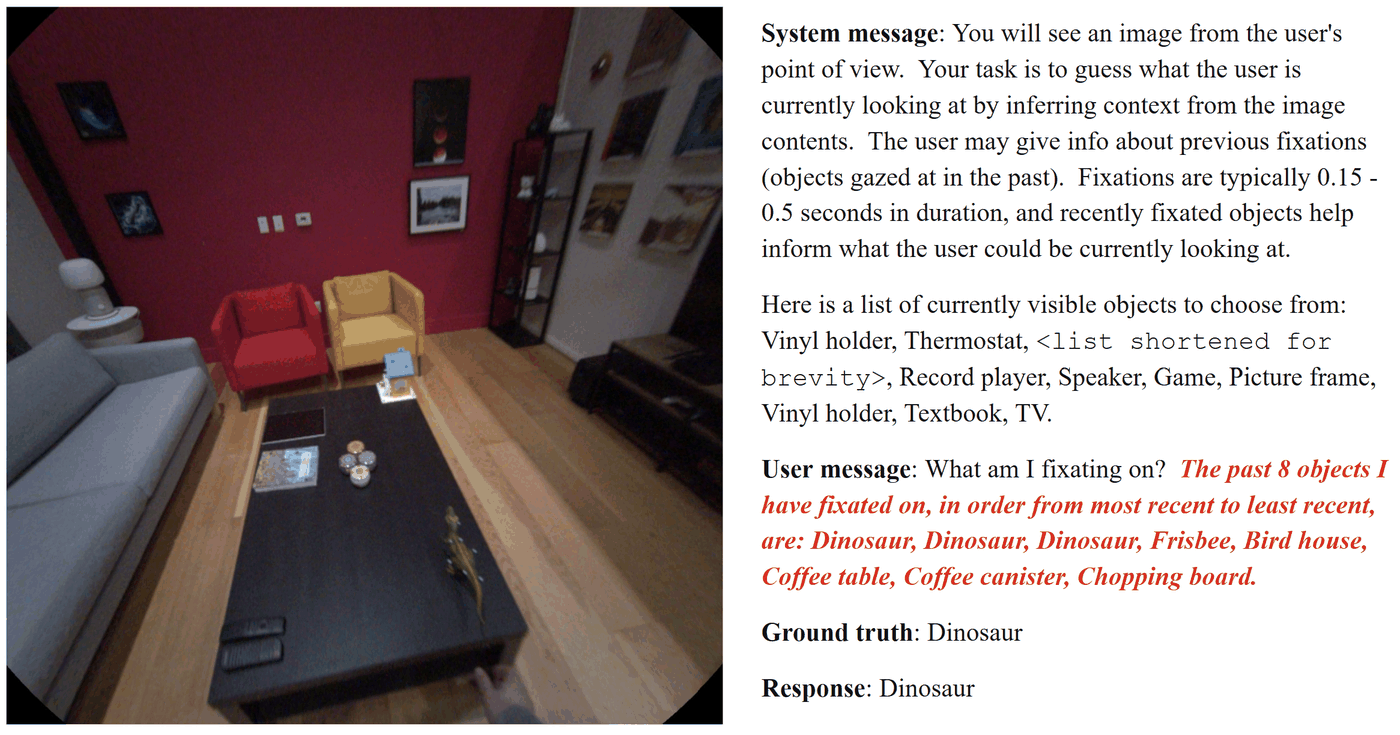
\includegraphics[width=0.9\linewidth]{figures/query_example.png}
    \caption{An example query to the VLM for E1.  The additional context from fixation history is highlighted in red; We vary the amount of context given to the model to measure how this context influences model understanding.}
    \label{fig:query_example}
\end{figure*}